\newif\ifglobal

%%%%%%%%%%%%%%%%%%%%%%%
%%% Compile to view %%%
%%%%%%%%%%%%%%%%%%%%%%%

%%%%%%%%%%%%%%%%%%%%%%%%%%%%%%%%%%%%%%%%%%%%%%%%%%%
%%% Readme:                                     %%%
%%% https://www.overleaf.com/read/bwdjvfjksvjy/ %%%
%%%%%%%%%%%%%%%%%%%%%%%%%%%%%%%%%%%%%%%%%%%%%%%%%%%

% >>> M?: marks a module setting number or important notice

% >>> M4: Set {./relative-path} to external files for this module <<<
\def \modulefiles {./17-EXTMEMENCR}
% To add an external file, use:
% (Replace '---' with actual filename)
% '\input{\modulefiles/tables/---.tex}' for tables
% '\includegraphics{\modulefiles/figures/---}' for figures
% '\subfile{\modulefiles/---}' for register files


% >>> M1: This module is in global project? <<<
% 'YES' - uncomment; 'NO' - comment out
\globaltrue

\ifglobal
    \documentclass[main\_\_CN.tex]{subfiles}

\else
    % Font "FandolSong-Regular" used by ctex does not have GSUB table.
    % It causes warnings that do not affect compilation and can be ignored.
    \PassOptionsToPackage{quiet}{fontspec}

    \documentclass[openany, 10pt]{book}

    % >>> M2: In ./00-shared/preamble-trm-module, also find
    %         settings for visibility of todo notes, watermark <<<
    \usepackage{preamble-trm-module}

    % Enable Chinese typesetting
    \usepackage{ctex}

    % >>> M3: Temporary labels in Chinese
    %         you can add your own labels there <<<
    \myexternaldocument{./00-shared/temp-labels-cn}

\fi %\ifglobal


\setcounter{secnumdepth}{4}


% >>> M5: If this module needs any updates in
% './00-shared/preamble-trm-module.sty'
% (include additional package, etc.), contact your module PM
% or create the file './00-shared/changelog.tex' make the
% necessary updates yourself and document them in this file <<<

% Make text left-aligned and allow latex to break pages naturally, comment out for full justification
\raggedright
\raggedbottom


\begin{document}


% Sets language into which pre-defined bits of text are translated
\selectlanguage{chinese}
\setchineseformatting


% Do not delete this block
\ifglobal
% Add the following front matter if
% this module is outside of global project
\else
    \InputIfFileExists{readme}{}{}
    \listoftodos
    {\let\clearpage\relax \listofdonetodos}
    \tableofcontents
    %\listoftables
    %\listoffigures
\fi


%%%%%%%%%%%%%%%%%%%%%%%%%
%%% TRM Module Begins %%%
%%%%%%%%%%%%%%%%%%%%%%%%%

\hypertarget{extmemencr}{}
\chapter{片外存储器加密与解密 (FLASH)}
\label{mod:extmemencr}


\section{概述}

ESP32 系列的多款芯片需要将程序和数据存储在片外 flash。片外 flash 可以用来存储专有软件、敏感的用户数据（比如用来访问私有网络的凭据）等。ESP32 的 flash 加密模块能够将代码进行加密，
然后将加密之后的代码写入片外 flash。
当 CPU 通过 cache 读片外 flash 时，flash 解密模块能够将读取到的指令和数据自动进行解密。ESP32 通过 flash 加解密模块为用户的应用代码提供了安全保障。


\section{主要特性}

\begin{itemize}
    \item 多种密钥生成方式
    \item 加密过程需要软件参与
    \item 高速的解密过程，无需软件参与
    \item 寄存器配置、系统参数、启动 (boot) 模式共同决定 flash 加解密功能
\end{itemize}


\section{功能描述}

\begin{figure}[H]
    \centering
    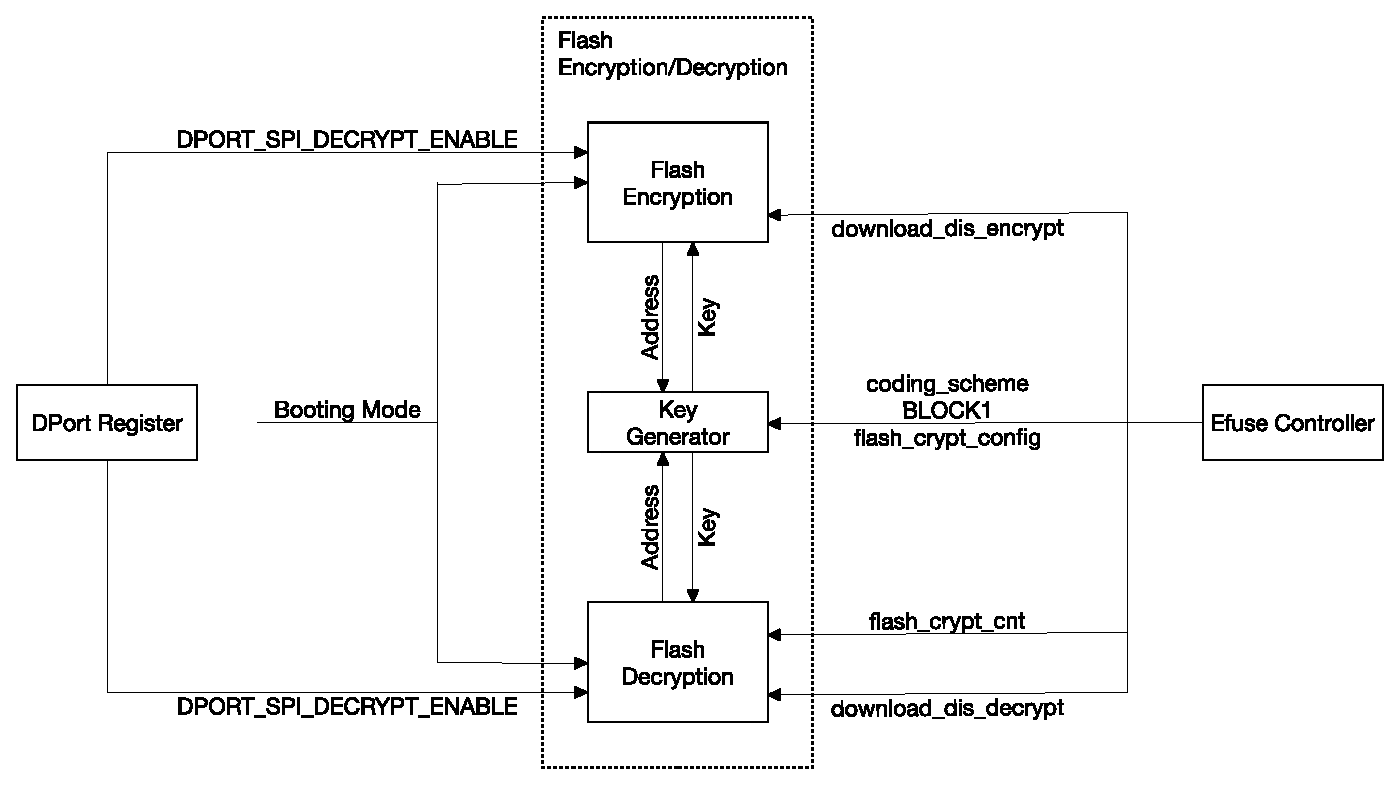
\includegraphics[width=1.0\textwidth]{./17-EXTMEMENCR/figures/Structure.eps}
    \caption{Flash 加解密模块架构}
    \label{figure:Structure}
\end{figure}

Flash 加解密模块包含三个部分，分别是密钥生成模块 (Key Generator)、flash 加密 (Flash Encryption) 模块和 flash 解密 (Flash Decryption) 模块，如图 \ref{figure:Structure} 所示。Key Generator 被 Flash Encryption 与 Flash Decryption 共同使用。Flash Encryption 与 Flash Decryption 可以同时工作。

外设 DPort 寄存器中与 flash 加解密相关的寄存器是 DPORT\_SLAVE\_SPI\_CONFIG\_REG 中的
DPORT\_SPI\_ENCRYPT\_ENABLE 位和 DPORT\_SPI\_DECRYPT\_ENABLE 位。Flash 加解密模块还会从外设 eFuse 控制器中获取 6 个系统参数，它们是 coding\_scheme、BLOCK1、flash\_crypt\_config、download\_dis\_encrypt、flash\_crypt\_cnt 和 download\_dis\_decrypt。


\subsection{Key Generator 模块}

Key Generator 首先依据系统参数 coding\_scheme、BLOCK1 生成\\
\begin{math}Key_{o} = f( coding\_scheme, BLOCK1 )\end{math}。

然后 Key Generator 根据系统参数 flash\_crypt\_config 和 flash 加解密模块访问的片外 flash 的实地址 \begin{math}Addr_{e}\end{math}、\begin{math}Addr_{d}\end{math} 分别运算出\\
\begin{math}Key_{e} = g( Key_{o}, flash\_crypt\_config, Addr_{e} )\end{math}、\\
\begin{math}Key_{d} = g( Key_{o}, flash\_crypt\_config, Addr_{d} )\end{math}。

当系统参数 flash\_crypt\_config 为全 0 时，
\begin{math}Key_{e}\end{math}、\begin{math}Key_{d}\end{math}
与片外 flash 的实地址无关。
当系统参数 flash\_crypt\_config 为除全 0 之外任意值时，
片外 flash 每 8 个 word 具有一个
其独特的 \begin{math}Key_{e}\end{math} 和 \begin{math}Key_{d}\end{math}。


\subsection{Flash Encryption 模块}

Flash Encryption 是一个外设模块，自身带有寄存器，这些寄存器可以被 CPU 直接访问。模块内的寄存器、外设 DPort 寄存器、系统参数、boot 模式共同配置并使用这一模块。

此模块工作时需要软件参与，其流程为：

\newcounter{STEP_W_ADDR}
\newcounter{STEP_POLL}
\newcounter{STEP_W_FLASH}
\begin{enumerate}
    \item 将寄存器 DPORT\_SLAVE\_SPI\_CONFIG\_REG 的 DPORT\_SPI\_ENCRYPT\_ENABLE 位置 1。
    \item 将准备写片外 flash 的实地址填入寄存器 FLASH\_ENCRYPT\_ADDRESS\_REG，
    此地址值必须是 8-word 对齐的。
    \setcounter{STEP_W_ADDR}{\theenumi}
    \item 将待加密的 8-word 代码中的最低地址的 word 填入寄存器 FLASH\_ENCRYPT\_BUFFER\_0\_REG，
    次低地址的 word 填入 FLASH\_ENCRYPT\_BUFFER\_1\_REG，
    以此类推直至填入 FLASH\_ENCRYPT\_BUFFER\_7\_REG。
    \item 将寄存器 FLASH\_ENCRYPT\_START\_REG 置 1。
    \item 轮询寄存器 FLASH\_ENCRYPT\_DONE\_REG，直到读到 1。
    \setcounter{STEP_POLL}{\theenumi}
    \item 调用函数，通过外设 SPI0 对片外 flash 的 8-word 对齐的地址写入任意 8-word 代码。
    \setcounter{STEP_W_FLASH}{\theenumi}
\end{enumerate}

步骤 1 至 \arabic{STEP_POLL} 操作 Flash Encryption 模块对 8-word 代码进行加密。
加密算法使用的密钥就是 \begin{math}Key_{e}\end{math}。
加密结果也是 8 个 word。
步骤 \arabic{STEP_W_FLASH} 操作外设 SPI0 将 Flash Encryption 的加密结果写入片外 flash。
步骤 \arabic{STEP_W_FLASH} 中调用的函数会有一个参数是写片外 flash 的实地址，
这个实地址必须是 8-word 对齐的，
且必须与步骤 \arabic{STEP_W_ADDR} 中填入寄存器 FLASH\_ENCRYPT\_ADDRESS\_REG 的值一致。
虽然步骤 \arabic{STEP_W_FLASH} 中调用的函数还会有一个参数是 8-word 代码，
但是在执行了步骤 1 至 \arabic{STEP_POLL} 的情况下，
这个参数无意义，外设 SPI0 此时使用的是加密后的结果。
若 Flash Encryption 处于未工作状态或者不执行步骤 1 至 \arabic{STEP_POLL}，
那么步骤 \arabic{STEP_W_FLASH} 不会使用加密结果而是函数中的参数。

Flash Encryption 是否处于工作状态取决于：

\begin{itemize}

    \item SPI Flash Boot 模式下

    当寄存器 DPORT\_SLAVE\_SPI\_CONFIG\_REG 的 DPORT\_SPI\_ENCRYPT\_ENABLE 位为 1 时，
    Flash Encryption 处于工作状态，
    否则处于未工作状态。

    \item Download Boot 模式下

    当寄存器 DPORT\_SLAVE\_SPI\_CONFIG\_REG 的 DPORT\_SPI\_ENCRYPT\_ENABLE 位为 1 且
    系统参数 download\_dis\_encrypt 为 0 时，
    Flash Encryption 处于工作状态，
    否则处于未工作状态。

\end{itemize}

虽然整个过程都有软件参与，
但是加密后的代码无法被软件直接读取。
加密后的代码被直接写到片外 flash 中。
虽然 CPU 可以不通过 cache 而直接读片外 flash 从而得到加密代码，
但软件还是绝对无法获取到密钥 \begin{math}Key_{e}\end{math}。


\subsection{Flash Decryption 模块}

Flash Decryption 并非外设模块，自身不带寄存器，因此不能被 CPU 直接访问。
外设 DPort 寄存器、系统参数、boot 模式共同配置并使用这一模块。

当此模块工作时，CPU 通过 cache 读取片外 flash 中的指令与数据。
Flash Decryption 将自动把读取到的指令与数据进行解密。
解密的整个过程无需软件参与并且对 cache 是透明的。
解密算法使用的密钥就是 \begin{math}Key_{d}\end{math}，
此密钥同样无法被软件获取。

当此模块未工作时，不对 flash 中的内容产生作用，无论是加密内容还是未加密内容，因此 CPU 通过 cache 读取到的是 flash 中的原始内容。

Flash Decryption 是否处于工作状态取决于：

\begin{itemize}

    \item SPI Flash Boot 模式下

    当系统参数 flash\_crypt\_cnt（7 bit 宽）中有奇数个 bit 为 1 时，
    Flash Decryption 处于工作状态，
    否则处于未工作状态。

    \item Download Boot 模式下

    当寄存器 DPORT\_SLAVE\_SPI\_CONFIG\_REG 的 DPORT\_SPI\_DECRYPT\_ENABLE 位为 1 且
    系统参数 download\_dis\_decrypt 为 0 时，
    Flash Decryption 处于工作状态，
    否则处于未工作状态。
\end{itemize}

\hypertarget{extmemencr-reg-summ}{}
\section{寄存器列表}
\label{sec:flash-reg-sum}

本小节的所有地址均为相对于片外存储器加密与解密 (FLASH) 基地址的地址偏移量（相对地址），具体基地址请见章节 \ref{mod:sysmem} \textit{\nameref{mod:sysmem}} 中的表 \ref{table:Peripheral_Address_Mapping}。

请查看章节 \hyperref[glossary-access-types]{\textit{寄存器的访问类型}}，了解“访问”列缩写的含义。

\begin{longtable}{ | p{6.5cm} | p{5cm} | p{2cm} | p{1cm} | }
\hline\rowcolor{lightgray}
名称 & 描述 &  地址 & 访问 \\ \hline
\hyperref[regdesc:FLASHENCRYPTIONBUFFERnREG]{FLASH\_ENCRYPTION\_BUFFER\_0\_REG} & Flash 加密 buffer 寄存器 0 & 0x3FF5B000 &只写 \\ \hline
\hyperref[regdesc:FLASHENCRYPTIONBUFFERnREG]{FLASH\_ENCRYPTION\_BUFFER\_1\_REG} & Flash 加密 buffer 寄存器 1 & 0x3FF5B004 & 只写 \\ \hline
\hyperref[regdesc:FLASHENCRYPTIONBUFFERnREG]{FLASH\_ENCRYPTION\_BUFFER\_2\_REG} & Flash 加密 buffer 寄存器 2 & 0x3FF5B008 &只写 \\ \hline
\hyperref[regdesc:FLASHENCRYPTIONBUFFERnREG]{FLASH\_ENCRYPTION\_BUFFER\_3\_REG} & Flash 加密 buffer 寄存器 3 & 0x3FF5B00C & 只写 \\ \hline
\hyperref[regdesc:FLASHENCRYPTIONBUFFERnREG]{FLASH\_ENCRYPTION\_BUFFER\_4\_REG} & Flash 加密 buffer 寄存器 4 & 0x3FF5B010 &只写 \\ \hline
\hyperref[regdesc:FLASHENCRYPTIONBUFFERnREG]{FLASH\_ENCRYPTION\_BUFFER\_5\_REG} & Flash 加密 buffer 寄存器 5 & 0x3FF5B014 & 只写 \\ \hline
\hyperref[regdesc:FLASHENCRYPTIONBUFFERnREG]{FLASH\_ENCRYPTION\_BUFFER\_6\_REG} & Flash 加密 buffer 寄存器 6 & 0x3FF5B018 & 只写 \\ \hline
\hyperref[regdesc:FLASHENCRYPTIONBUFFERnREG]{FLASH\_ENCRYPTION\_BUFFER\_7\_REG} & Flash 加密 buffer 寄存器 7 & 0x3FF5B01C & 只写 \\ \hline
\hyperref[regdesc:FLASHENCRYPTIONSTARTREG]{FLASH\_ENCRYPTION\_START\_REG} & 加密操作控制寄存器 & 0x3FF5B020 & 只写 \\ \hline
\hyperref[regdesc:FLASHENCRYPTIONADDRESSREG]{FLASH\_ENCRYPTION\_ADDRESS\_REG} & 片外 flash 地址寄存器 & 0x3FF5B024 & 只写 \\ \hline
\hyperref[regdesc:FLASHENCRYPTIONDONEREG]{FLASH\_ENCRYPTION\_DONE\_REG} & 加密操作状态寄存器 & 0x3FF5B028 & 只读 \\ \hline

\end{longtable}
\section{寄存器}

本小节的所有地址均为相对于片外存储器加密与解密 (FLASH) 基地址的地址偏移量（相对地址），具体基地址请见章节 \ref{mod:sysmem} \textit{\nameref{mod:sysmem}} 中的表 \ref{table:Peripheral_Address_Mapping}。寄存器绝对地址见章节 \ref{sec:flash-reg-sum} \textit{\nameref{sec:flash-reg-sum}}。

关于保留 (reserved) 域的处理，请查看章节 \hyperref[programming-reserved-field]{\textit{如何配置寄存器的保留域}}。

\subfile{\modulefiles/flashenc_reg_cn.tex}

\end{document}
